\documentclass[conference,11pt,twocolumn,twoside,a4paper]{IEEEtran}
\IEEEoverridecommandlockouts

\usepackage[verbose,expansion=alltext,stretch=50]{microtype}
\usepackage{datetime}
\usepackage{graphicx}
\usepackage{booktabs}
\usepackage[hidelinks]{hyperref}
\usepackage{subcaption}
\usepackage[labelformat=parens,labelsep=quad,skip=3pt]{caption}
\usepackage{fancyhdr}
\usepackage[textwidth = 155mm]{geometry}
\usepackage[table,xcdraw]{xcolor}
\usepackage[english]{babel}
\usepackage[backend=biber,style=numeric,sorting=ynt]{biblatex}
\usepackage{textpos}
\usepackage{color}
\usepackage{listings}
\usepackage{tablefootnote}

\addbibresource{report.bib}

\newcommand{\link}[1]{{\color{blue}\href{#1}{#1}}}
\newcommand{\email}[1]{{\href{mailto:#1}{#1}}}

\newcommand{\titleText}{Text Independent Writer Recognition Using LBPH \& SVM}
\newcommand{\course}{CMP450 -- Semester 20/21}
\newcommand{\teamname}{Team \#1}

\graphicspath{ {./figures/} }

\title{\normalsize{\course} \\\Huge{\titleText} \\\vspace*{7pt} \normalsize{\today}}

\author{
    \LARGE{\teamname}\\
    \IEEEauthorblockN{
      \normalsize{Mahmoud Othman Adas} \small{\texttt{SEC:2, BN:19}\IEEEauthorrefmark{1}} and
      \normalsize{Yosry Mohamed Yosry} \small{\texttt{SEC:2, BN:33}\IEEEauthorrefmark{2}} and \\
      \normalsize{Ahmad Mahmoud AbdElMen'em Afifi} \small{\texttt{SEC:1, BN:5}\IEEEauthorrefmark{3}} and
      \normalsize{Abdulrahman Khalid Hassan} \small{\texttt{SEC:1, BN:30}\IEEEauthorrefmark{4}}
    }
    \IEEEauthorblockA{
        \\Department of Computer Engineering,
        Cairo University\\
        Email: 
        \IEEEauthorrefmark{1}\email{mahmoud.ibrahim97@eng-st.cu.edu.eg},
        \IEEEauthorrefmark{2}\email{yosry.mohammad99@eng-st.cu.edu.eg}, \\
        \IEEEauthorrefmark{3}\email{Ahmed.Afifi98@eng-st.cu.edu.eg},
        \IEEEauthorrefmark{4}\email{abdulrahman.elshafie98@eng-st.cu.edu.eg}
    }
}

\pagestyle{fancy}
\fancyhf{}
\rhead{\course}
\lhead{\teamname}
\cfoot{\thepage}

% Default fixed font does not support bold face
\DeclareFixedFont{\ttb}{T1}{txtt}{bx}{n}{12} % for bold
\DeclareFixedFont{\ttm}{T1}{txtt}{m}{n}{12}  % for normal

% Custom colors
\definecolor{deepblue}{rgb}{0,0,0.5}
\definecolor{deepred}{rgb}{0.6,0,0}
\definecolor{deepgreen}{rgb}{0,0.5,0}

\lstdefinestyle{python}{
  belowcaptionskip=1\baselineskip,
  breaklines=true,
  xleftmargin=\parindent,
  keywordstyle=\bfseries\color{green!40!black},
  commentstyle=\itshape\color{purple!40!black},
  identifierstyle=\color{blue},
  numbers=left,
  numberstyle=\tiny\color{gray},
  captionpos=b,
  language=Python,
  basicstyle=\ttm,
  otherkeywords={self},             % Add keywords here
  keywordstyle=\ttb\color{deepblue},
  emph={MyClass,__init__},          % Custom highlighting
  emphstyle=\ttb\color{deepred},    % Custom highlighting style
  stringstyle=\color{deepgreen},
  frame=tb,                         % Any extra options here
  showstringspaces=false            % 
}

% Example:
% \lstset{escapechar=@,style=python,caption={some caption.},label=list:example}
% \begin{lstlisting}
% class Habal():
%   def __init__(self):
%     print('hello')
% \end{lstlisting}

\begin{document}
    \maketitle
    \thispagestyle{plain}

    \section{Introduction}
% TODO    
    \section{Pipeline}
% TODO summary of the pipeline
    \section{Preprocessing Module}
% TODO
    \section{Feature Extraction Module}
The feature extraction module is to extract features to be able to distinguish one writer from the other.

We chose Local Binary Patterns as our feature extractor to extract features from the gray images of lines of each writer; LBP is a texture descriptor used to extract features by computing a local representation by comparing each pixel with its surrounding neighbors.

The first step in constructing the LBP texture descriptor is to convert the image to grayscale. We select a neighborhood of size r surrounding the center pixel for each pixel in the grayscale image. An LBP value is then calculated for this center pixel and stored in the output 2D array with the same width and height as the input image.

% figure 1
Figure \ref{fig:lbp_thresholding} The first step in constructing a LBP is to take the 8 pixel neighborhood surrounding a center pixel and threshold it to construct a set of 8 binary digits.

\begin{figure}
    \centering
    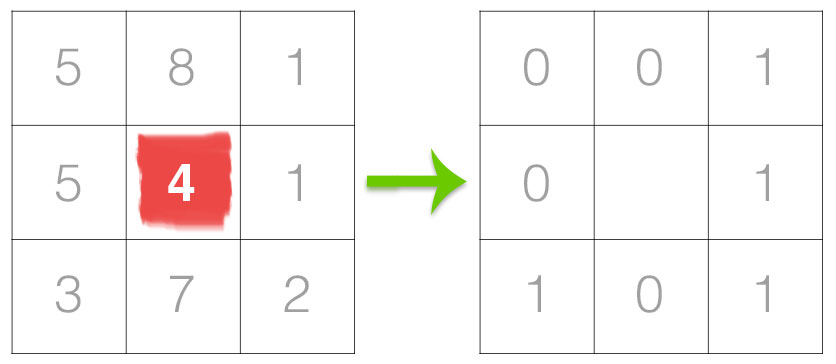
\includegraphics[width=0.9\linewidth]{../figures/lbp_thresholding.jpg}
    \caption{Constructing a set of 8 binary digits from the 8 neighbours surrounding the center.}
    \label{fig:lbp_thresholding}
\end{figure}

In this figure, the center colored by red, LBP checks if the intensity of the center pixel is greater-than-or-equal to its neighbor, then we set the value to 1; otherwise, we set it to 0

The second step is to calculate the LBP value for the center pixel by list the eight binary digits we got in the previous step and convert it to decimal, and we should list the binary digits by the same order and direction for every pixel in the dataset.

% figure 2
Figure \ref{fig:lbp_calculation} The Second step is taking the 8-bit binary neighborhood of the center pixel and converting it into a decimal.

\begin{figure}
    \centering
    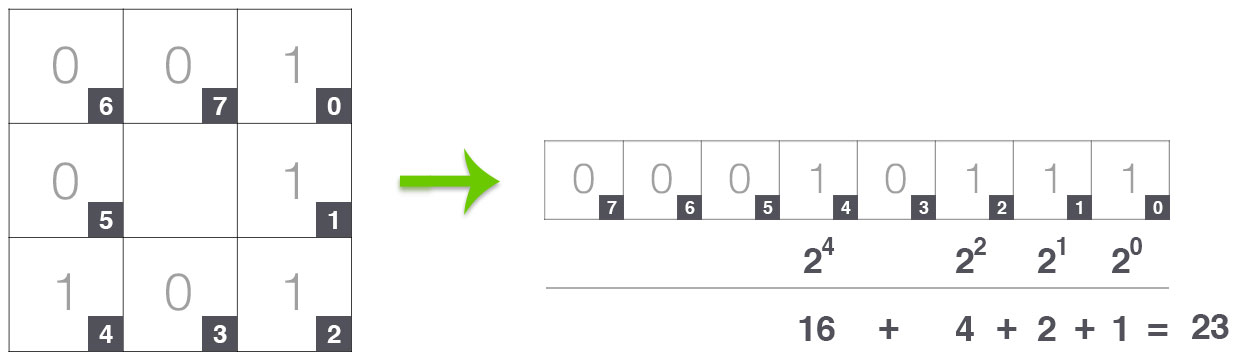
\includegraphics[width=0.9\linewidth]{../figures/lbp_calculation.jpg}
    \caption{Taking the 8-bit binary neighborhood of the center pixel and converting it into a decimal value.}
    \label{fig:lbp_calculation}
\end{figure}

% figure 3
Figure \ref{fig:lbp_to_output} Finally, yielding the LBP value and store it in the LBP output image.
\begin{figure}
    \centering
    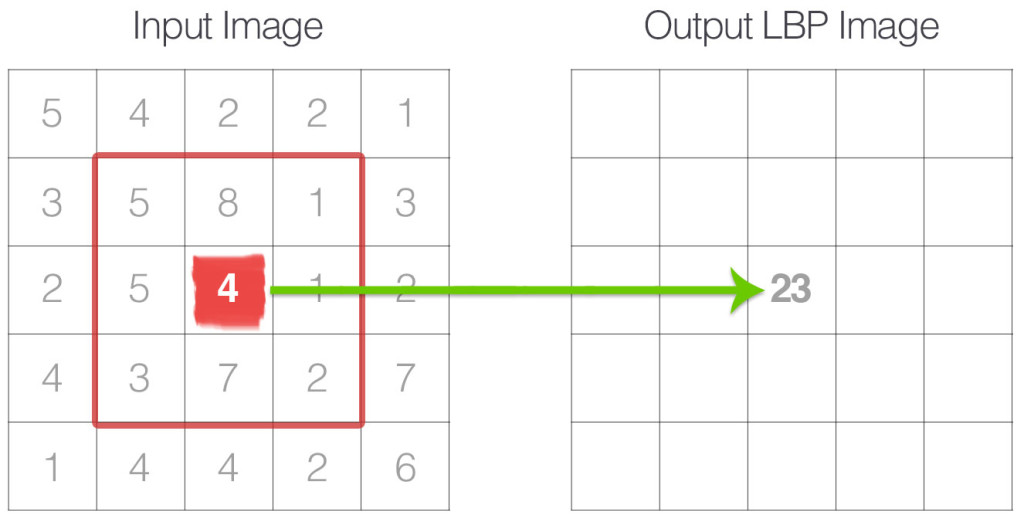
\includegraphics[width=0.9\linewidth]{../figures/lbp_to_output.jpg}
    \caption{The calculated LBP value is then stored in an output LBP image.}
    \label{fig:lbp_to_output}
\end{figure}

By fine-tuning the parameters of LBP such as the number of points \texttt{p} in a circularly symmetric neighborhood and the radius of the circle \texttt{r}
We chose radius equals 3 and 8 neighbors as it gives us the sweet spot between accuracy and speed. Another acceptable parameter will be four neighbors with a radius of 3. It also works very well with a little dropdown in the accuracy and less calculation time.
After calculating the LBP image, we get our feature vector by taking its histogram as our feature vector, and by trials, we found out that masking it with the binary image to calculate only the histogram for the black pixels in the binary image gives us better accuracy.
Moreover, because we have eight neighbors, we got $2 ^ 8 = 256$ possible patterns, so our LBP image has a minimum value of 0 and a maximum value of 255, allowing us to construct a 256-bin histogram of LBP codes as our final feature vector.
Finally, we normalize our feature vector by dividing it by its means.
    \section{Classification Module}
The classification module aims to train the features extracted from handwritten samples from the three different writers with their labels, then trying to predict the test handwritten sample's writer.

After research we chose support vector machine, SVM for short, to be our classification module as it has lots of pros we need such as:
\begin{itemize}
    \item It has lots of pros, such as it is useful in cases where the number of dimensions is greater than the number of samples.
    \item It uses a subset of training points in the decision function. Hence, it is memory efficient.
    \item It is useful in high dimensional spaces.
\end{itemize}

The SVM algorithm's objective is to find a hyperplane that distinctly classifies the data points in an N-dimensional space where \texttt{N} is the number of features.

We are using a \texttt{sigmoid} kernel with penalty parameter \texttt{C=1} and \texttt{ovo} decision function.
Furthermore, after fitting the training images' features with their labels, we use the SVM to predict the writer from the test image features.

    \section{Speed Enhancements}
We put a lot of effort on speeding up the our system's pipeline.
The most effective optimization was parallelizing the feature extraction by extracting each image's features in a separate process and then collecting all the features before training.

Processes are quite heavy, but python threads are totally useless, thanks to \texttt{GIL}'s locking mechanism.
We believe that if we port the code to another language, the execution time would be much lower using threads and manual memory allocation.

Python lists are known to be very slow, so we replaced them all with numpy arrays, and allocated most of the needed memory ahead before the system starts operating on the images.
A quite speed gain came from fine tuning \texttt{skimage} and \texttt{OpenCV} parameters.

We tried to use \texttt{Numba} and \texttt{Cython} to optimize the execution time but they didn't have an effect.
It was probably because most of the code calls numpy, \texttt{skimage} and \texttt{OpenCV}, which are all written in C and well optimized for memory and CPU.
    \section{Performance Analysis}
% TODO
    \section{Unsuccessful Trials}
We started with and settled on using \texttt{LBPH} for feature extraction and \texttt{SVM} for classfication.
They both gave around 80\% accuracy at the beginning, and with tuning for preprocessing the accuracy reached \~99\% over large tests.
During that, part of the team were testing other feature extraction methods and classfiers.

We tried to extract \emph{Histogram of Oriented Gradients} (\texttt{HOG}) features.
Using \texttt{HOG} gave very low accuracy (\~46\%) on 15 test cases.
We extracted \texttt{HOG} from the binary image and then gray image, with no visible changes.

Then we tried to extract the \emph{Hu Moments} that are used to describe the shapes.
We extracted \emph{Hu Moments} from each binary line in the image.
Using \emph{Hu Moments} with \texttt{SVM} gave accuracies lower than that of \texttt{HOG} on the same number of test cases.

Being very low made sense, because we tried to describe the shape of the whole line.
So we tried to extract \emph{Hu Moments} from a sliding window of size $13\times13$.
This gave accuracy of \~48\% on 15 tests.
On some lucky iterations, it gave \~80\%.

Then we tried to mix both \texttt{HOG} features and \emph{Hu Moments}.
This gave us accuracy of \~66\% on 15 tests.
It wasn't slower than only \texttt{HOG}, because we used subset of both features.

By this time, \texttt{LBPH} reached \~99\% accuracy on 200 tests.
So we abandoned optimizing the feature extraction anymore.

Figure \ref{fig:unsuccBar} shows the accuracies for the different features.

\begin{figure}
    \centering
    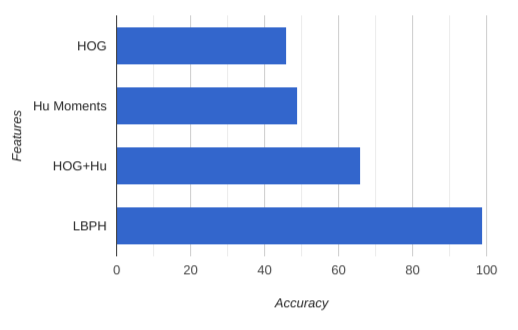
\includegraphics[width=0.9\linewidth]{unsuccBar}
    \caption{Feature Extraction Methods Accuracy for 15 tests.}
    \label{fig:unsuccBar}
\end{figure}

We tried another classfication method beside \texttt{SVM}.
We used \emph{K-Nearest Neighbours} (\texttt{KNN}), and it gave the same accuracies of \texttt{LBPH} but was noticably slower.
It made sense that \texttt{KNN} is slower, because it iterates over the features multiple times to find the mean and cluster them.

    \section{Future Work}
In an upcoming work, we could try generalizing our system on different forms of handwritten text by working on other datasets. Other features (in combination with \texttt{LBPH}) could be explored if \texttt{LBPH} was not enough to produce high accuracy on other forms of handwritten text. We used \texttt{scikit-image}'s implementations of LBP to construct our feature vector. Other implementations could be explored in the hope of finding a more efficient implementation. We parallelized feature extraction of different images on different processors to lower processing time. If images must be processed sequentially, we could try parallelizing the calculations of LBP for each line in an image, then collecting the results to construct the LBP histogram.
    \section{Workload Distribution}

\subsection{Mahmoud Othman Adas}
\begin{itemize}
    \item TODO
\end{itemize}

\subsection{Yosry Mohamed Yosry}
\begin{itemize}
    \item TODO
\end{itemize}

\subsection{Ahmad Mahmoud AbdElMen'em Afifi}
\begin{itemize}
    \item TODO
\end{itemize}

\subsection{Abdulrahman Khalid Hassan}
\begin{itemize}
    \item TODO
\end{itemize}

    \section{Conclusion}
% TODO

    \printbibliography
\end{document}
